
%\chapter{Přirozené experimenty}\label{Prirozene_experimenty}
\chapter{Senátní volby jako přirozený experiment}\label{Prirozene_experimenty}

\textit{René Levínský, Ján Palguta, Samuel Škoda}

\section*{Úvod}
Chceme-li zkoumat vliv jednotlivých nefarmaceutických opatření (jako je např. otevření či uzavření škol) na vývoj epidemie, narážíme vždy na stejný problém, a sice na nemožnost zorganizovat náhodný experiment s~kontrolní skupinou. 

Smyslem režimových opatření je řízení epidemie. Je třeba je regionálně přijímat dle vývoje epidemie -- zpřísňovat je v~zasažených oblastech a uvolňovat v~částech země, kde epidemie opadá. V~žádném případě tedy nelze režimová opatření v~jednotlivých oblastech zavádět náhodně, tedy tak, jak organizujeme běžné experimenty. Není to prvotně problém technický či organizační, jistě bychom mohli pro každý okres ČR provést hod mincí a v~případě, padne-li panna, v~daném okrese např. zavřít obchody (padl-li by orel, obchody by zůstaly otevřené). Odhlédneme-li od reálných limit takového experimentu (mezi které patří např. pohyb obyvatel mezi jednotlivými oblastmi) i od morálních aspektů takového experimentu (těžko bychom hledali etickou komisi, která by takový experiment schválila), provedení takového experimentu je v~přímém rozporu s~podstatou právního státu. Je vyloučeno, aby soudní moc libovolného právního státu schválila omezení práv svých občanů na základě hodu mincí.

Naštěstí existují experimenty přirozené, tedy takové, v~nichž je země rozdělena náhodně, nezávisle na průběhu epidemie, a sice na základě pravidel, která byla schválena v~jiném historickém kontextu. Takovým přirozeným experimentem bylo v~České republice 2. kolo voleb do Senátu Parlamentu České republiky. Zatímco první kolo senátních voleb proběhlo společně s~volbami do krajských zastupitelstev (kromě několika pražských senátních obvodů tedy volila celá Česká republika), druhé kolo proběhlo pouze ve 26 z~81 senátních obvodů. (Každé dva roky je volena třetina, tedy 27 senátorů, nicméně senátor Zbyněk Linhart byl na podzim 2020 zvolen v~obvodě č. 33 -- Děčín již v~prvním kole). Rozdělení obvodů na jednotlivé třetiny 
%(viz. obr. 
proběhlo v~roce 1995, nemá žádnou souvislost s~epidemií covid-19. 

\begin{figure}[ht]
    \begin{center}
    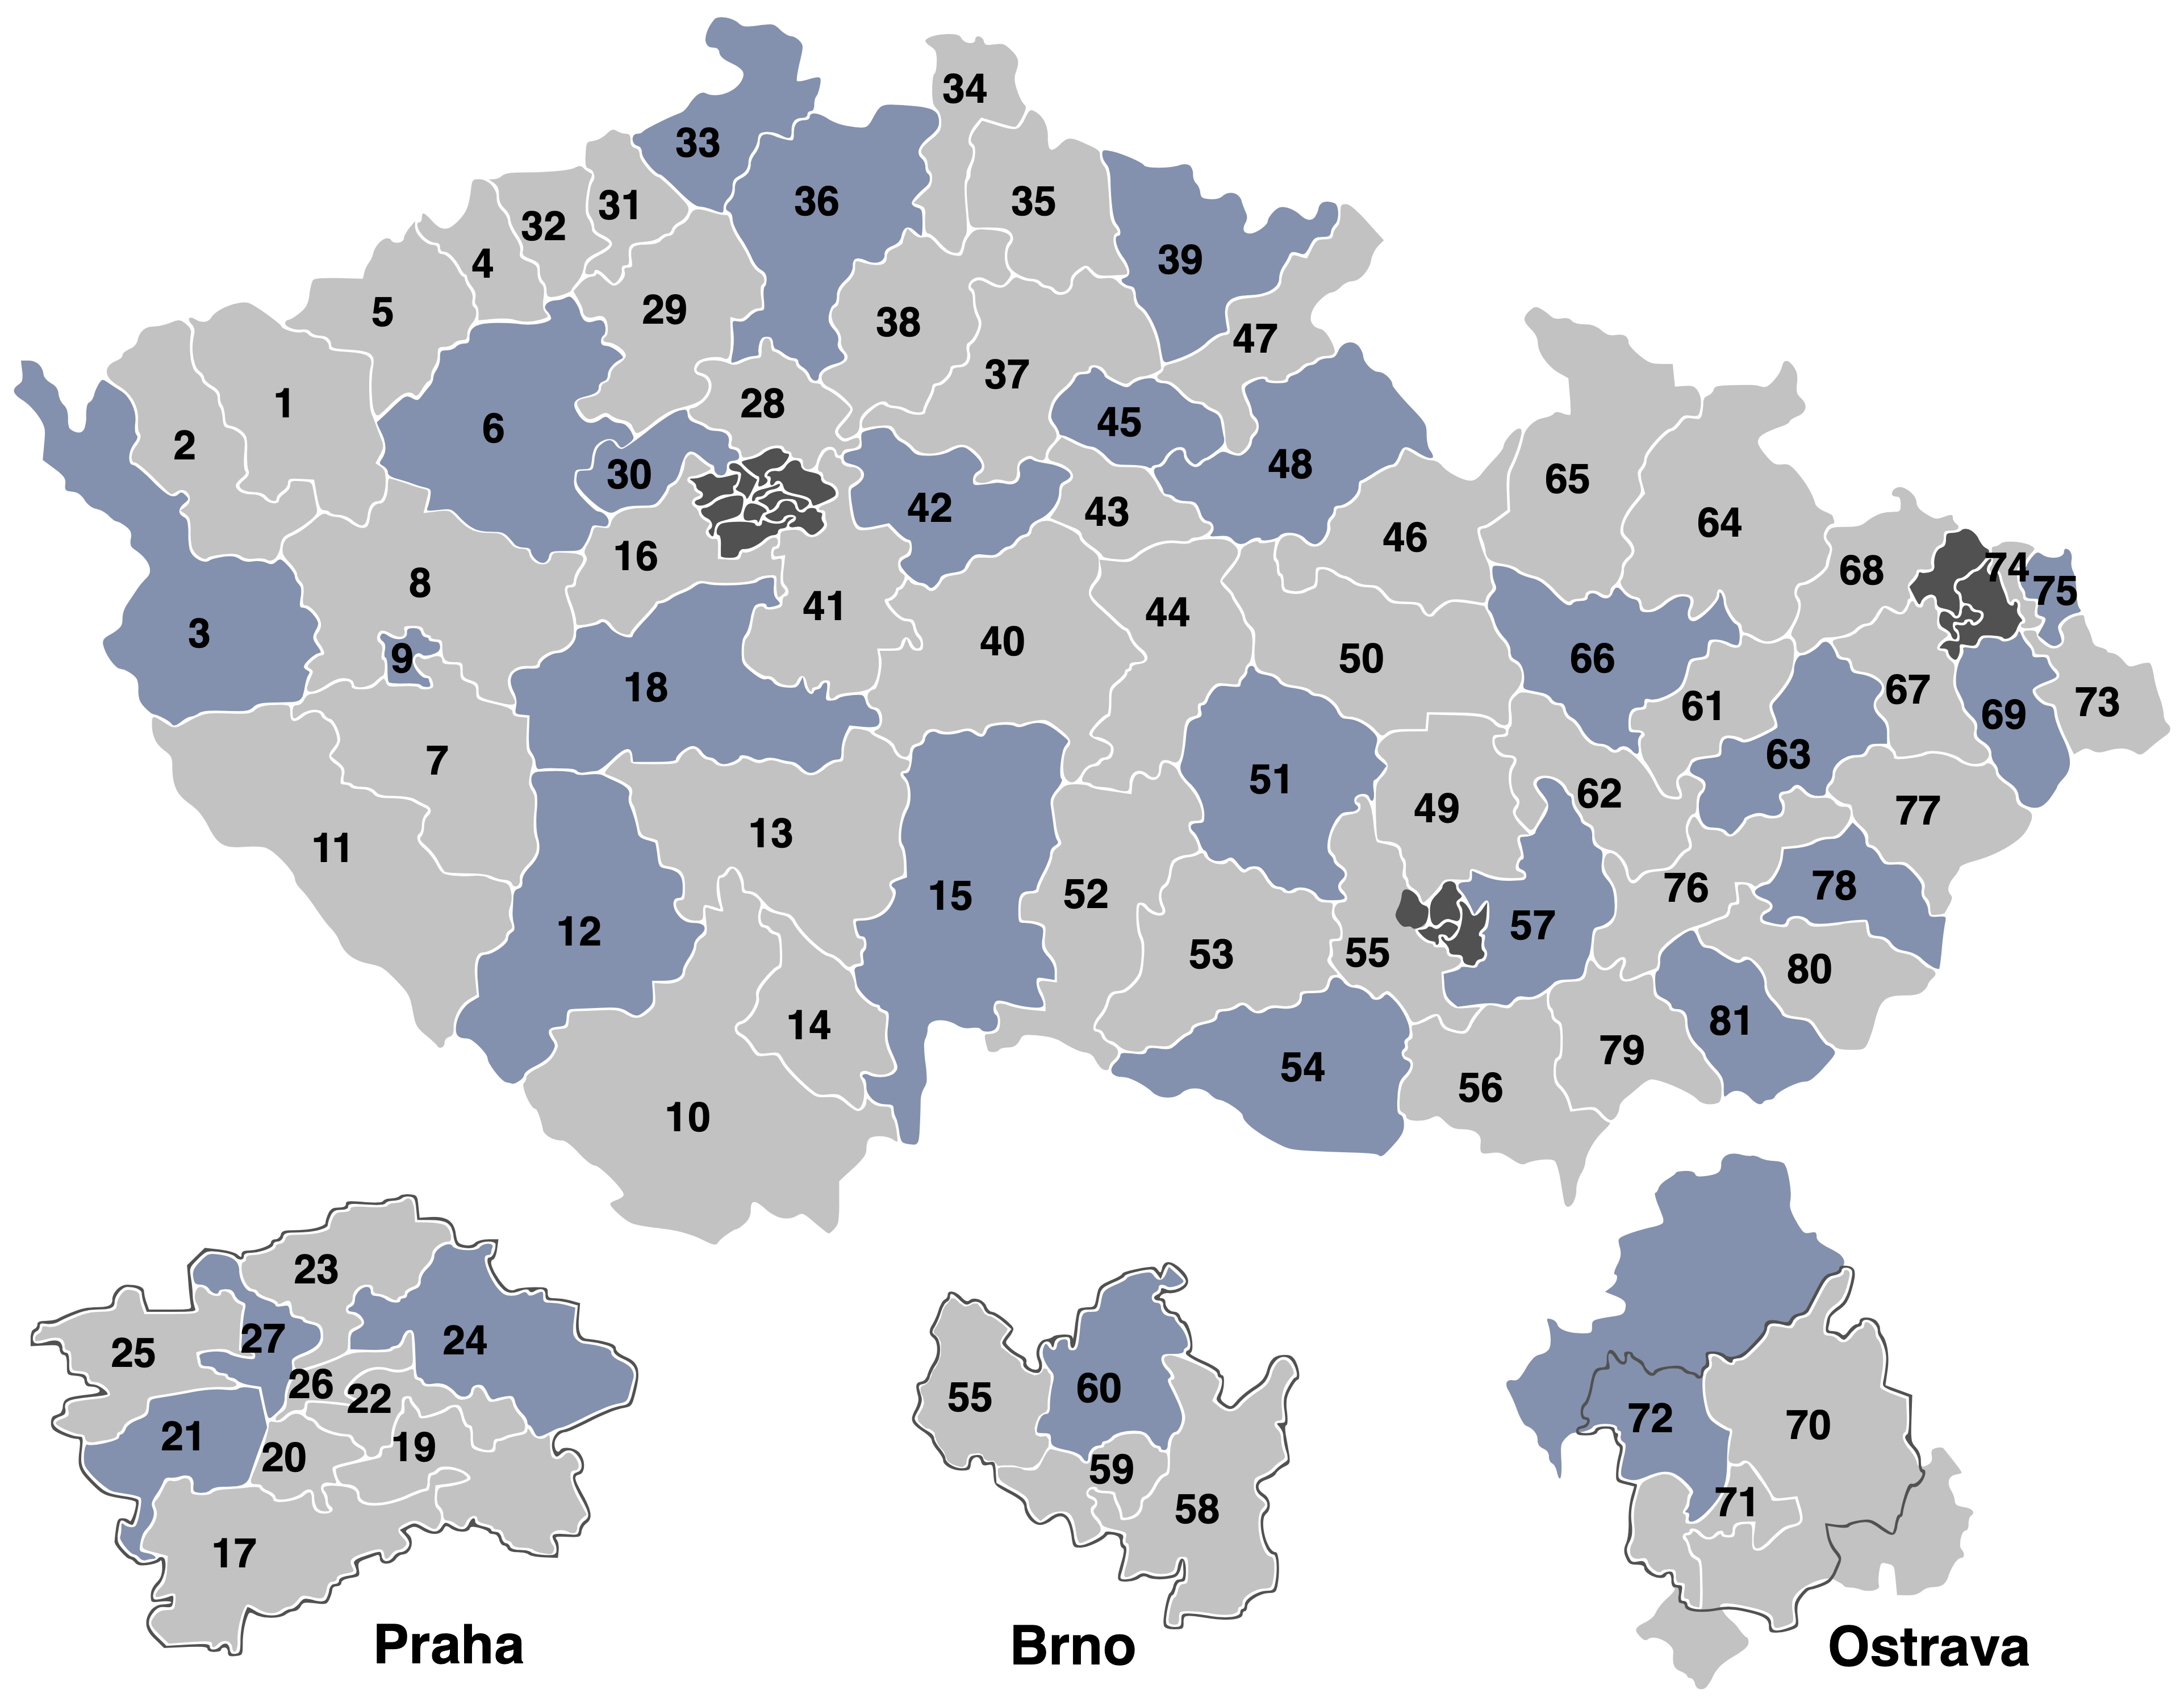
\includegraphics[scale=0.065]{okrsky_v3.png}
    \label{fig:senate_map}
    \end{center}
    \smallskip
    \caption{Mapy volebních obvodů pro volby do Senátu Parlamentu ČR. Na podzim 2020 proběhly volby pouze ve volebních obvodech 3, 6, 9, 12, ... (modře).}
    \end{figure}

Druhé kolo senátních voleb se tak \uv{shodou okolností} stalo přirozeným experimentem, ideální příležitostí, jak ověřit míru vlivu rozsáhlé akce, které se účastní stovky tisíc lidí, na vývoj epidemie.

Náš pokus o~odhad vlivu voleb na vývoj epidemie covid-19 samozřejmě není první, tímto tématem se zabývali vědci v~mnoha zemích. Nejstarší články, které zkoumaly vliv voleb na růst nových infekcí a mortalitu \cite{Berry2020, feltham2020no, AJPH2020}, nepotvrdily obavy, že by volby přispívaly k~růstu epidemie covid-19. Otázkou však zůstává, do jaké míry jsou realistické modely, které v~daných článcích odhadují vývoj epidemie v~hypotetickém případě neuskutečnění voleb. Dalším problémem je relativní homogenita volební účasti ve všech studovaných případech. Na druhou stranu, 
\cite{bertoli_france}, \cite{cotti2020relationship} i \cite{Cassan2020} 
ukazují, v~ostrém protikladu k~výše citovaným studiím, že volby signifikantně zrychlují růst epidemie. Tyto rozporuplné výsledky jsou dalším důvodem, proč studovat vliv voleb pomocí přirozeného experimentu, v~němž není třeba hypotetický svět \uv{bez voleb} modelovat, neboť tento svět v~dané zemi (ve smyslu kontrolní skupiny) existuje.\footnote{Podobně debata probíhá i v~případě dalších událostí s~politickým pozadím, jako jsou např. velká volební setkání. Např. \cite{dave2020risk} používají umělou kontrolní skupinu, s~jejíž pomocí ukazují, že široce kritizovaná Trumpova setkání s~voliči v~Tulse a Oklahomě nejspíše nezpůsobila zásadní růst nových případů covid-19 ani růst mortality. Na druhou stranu  \cite{bernheim2020effects} agregují 18 Trumpových volebních setkání a odhadují, že tato setkání způsobila 30 tisíc případů covid-19 a přibližně 700 úmrtí.  \cite{bernheim2020effects} ukazují dále, že vliv jednotlivých setkání je velice různorodý a analýzu setkání jediného, jako bylo třeba to v~Tulse, není možno považovat za reprezentativní}


\section*{Metodologie}
Je zřejmé, že k~zodpovězení naší výzkumné otázky potřebujeme model, který by (i) porovnal průběh epidemie ve volebních a nevolebních obvodech před druhým kolem senátních voleb a (ii) odhadl {\it volební efekt} jako rozdíl v~povolební dynamice vývoje epidemie.

Pokud by byla nákaza pozorovatelná okamžitě u~všech nakažených (perfect monitoring), viděli bychom rozdíl mezi volebními a nevolebními okrsky okamžitě v~den voleb. Skutečnost je ovšem samozřejmě jiná, nákazy vidíme s~odstupem, který navíc není pevně daný, a to jak kvůli rozdílné inkubační době mezi jedinci, tak kvůli různému časovému odstupu testování. Pozorovaný rozdíl v~incidenci tak nemůže být jednorázový, nicméně jde o~poměrně krátkou periodu. Ve chvíli, kdy se mezi detekovanými přestanou objevovat ti, kteří se nakazili ve volební den (ať už ve volebním či nevolebním obvodu), růst epidemie ve volebních a nevolebních obvodech se opět vyrovná (jakkoli růst epidemie ve volebních obvodech bude pravděpodobně z~jiného základu). V~případě, že jisté, dané procento nakažených bude potřebovat nemocniční péči, bychom ve volebních obvodech měli pozorovat jiný (vyšší) růst počtu hospitalizovaných.  

Formálně modelujeme růst pandemie následovně
%\begin{eqnarray}
\begin{equation}
\label{eq:event_study}
\frac{P_{t,m} - P_{t-n,m}}{P_{t-n,m}} = \sum_{j=-J}^{K} \beta_j \textit{Elections}_m \times Day_j + \textbf{X}_{m,t-n}^{'}\Gamma + \lambda_{m} + \lambda_{t} + \varepsilon_{m,t}
\end{equation}
\begin{equation}
\label{eq:event_study2}
\frac{H_{t,r} - H_{t-n,r}}{H_{t-n,r}} = \sum_{j=-J}^{K} \delta_j \textit{Elections share}_r \times Day_j + \textbf{X}_{r,t-n}^{'}\Gamma + \lambda_{r} + \lambda_{t} + \epsilon_{r,t}
\end{equation}

Základní proměnné, které chceme vysvětlit, jsou relativní růsty za $n$ dní, a to růst prevalence $P$ v~rovnici (\ref{eq:event_study}) a růst počtu hospitalizovaných v~rovnici (\ref{eq:event_study2}), které pozorujeme v~obci $m$ (v~případě prevalencí), či v~obci s~rozšířenou působností $r$ (v~případě hospitalizací) v~den $t; \beta$ a $\Gamma$ jsou odhadované koeficienty.\footnote{$n$ položíme rovno 14 dnům, takže zkoumaná perioda růstu obsahuje
(i) bezpříznakovou inkubační dobu\cite{lauer_et_al2020}, (ii) čas potřebný pro rezervaci testu, test samotný a jeho vyhodnocení (iii) případnou hospitalizaci. Abychom ověřili robustnost studie, budeme pracovat i se sedmidenním růstem incidence, který též vyrovnává kolísání v~rámci týdne.}


V~rovnici~(\ref{eq:event_study}) jsou předmětem našeho zájmu proměnné, které získáme jako součin binárního indikátoru udávajícího, zda se v~dané oblasti v~roce 2020 volby konaly, a dummy proměnné pro jednotlivé dny $j$, kde $j$ nabývá hodnot od $-J$ do $K$. 
Dobu před volbami zkoumáme pro $J=28$ dní, což je doba dostatečně dlouhá na to, abychom byli schopni detekovat případné rozdíly mezi volebními a nevolebními oblastmi v~době před konáním voleb. Povolební období pak budeme zkoumat po dobu $K=56$ dní, tedy opět po dobu, během níž by se projevil jakýkoli vliv voleb na pandemii. Abychom postihli nelineární podstatu pandemie, zavedeme dále časově závislé kontrolní proměnné $\textbf{X}_{m,t-n}$, které popisují pandemickou situaci v~dané obci $n$ dní před časem $t$ (např. kumulativní počet případů, příp. počet aktivních případů). Dále model obsahuje fixní efekt pro každou obci $\lambda_{m}$ a fixní efekt pro každý den $\lambda_{t}$, neboť musíme uvážit časovou i geografickou heterogenitu pandemického trendu. Chybový člen značíme
 $\varepsilon_{m,t}$.

V~regresi nemocničních případů~(\ref{eq:event_study2}) jsou našimi zkoumanými proměnnými součiny podílu počtu obyvatel daného ORP ve volební oblasti a opět dummy proměnné pro jednotlivé dny $j$, kde $j$ nabývá hodnot od $-J$ do $K$.\footnote{Ve třech největších městech -- v~Praze, Brně a Ostravě -- uvažujeme o~všech obyvatelích jako o~těch, kteří žijí ve volebním obvodu, neboť \textit{de facto} tvoří jedinou obec provázanou mnoha vazbami. Naše analýza je nicméně robustní ve smyslu, že stejné výsledky dostáváme i v~případě, že také v~těchto městech bereme počet obyvatel ve volebním okrsku úměrný části voličů, která je ve skutečnosti oprávněna volit.} Důvod tohoto postupu je prostý -- některá ORP jsou rozdělena mezi jednotlivé senátní obvody, takže se může stát, že některá obec v~rámci stejného ORP \uv{volí} a některá ne. Dále model obsahuje fixní efekt pro každou obci $\lambda_{r}$ a fixní efekt pro každý den $\lambda_{t}$, stejně jako v~předešlé rovnici. Chybový člen značíme $\varepsilon_{r,t}$.

\subsection*{Data}
\paragraph{Epidemiologická data.}  Veřejná data Ministerstva zdravotnictví ČR a Ústavu pro zdravotnické informace a statistiku (ÚZIS) popisují epidemiologickou situaci ve všech 6259 obcích České republiky. Pro každou obec udávají denní počet nových detekovaných případů, a to jak celkem, tak separátně v~kategorii nad 65 let. Dále tato data obsahují informace o~hospitalizovaných a pozitivitě PCR testů separátně pro všech 206 obcí s~rozšířenou působností (ORP). 

\paragraph{Sociodemografická data.} 
Pokud rozdělujeme populaci ve volebních a nevolebních obvodech podle věku či jiných sociodemografických hledisek, pak používáme data ze Sčítání lidu v~roce 2011. Veřejně přístupná data jsou Českým statistickým úřadem (ČSÚ) poskytována na úrovni obcí.

\section*{Výsledky}
Nejprve porovnejme růst nových případů ve volebních a nevolebních okrscích. Na panelu A~obrázku \ref{fig:Covid_growth14}  jsou znázorněny průměrné čtrnáctidenní přírůstky ve volebních a nevolebních obvodech v~průběhu druhého kola senátních voleb na podzim 2020. Zatímco vývoj epidemie v~časovém úseku před 2. kolem senátních voleb
je ve volebních a nevolebních obvodech velice podobný, na první pohled vidíme odlišný čtrnáctidenní růst epidemie v~období 2 až 3 týdnů po volbách. Panel B pak zobrazuje odhadnuté rozdíly mezi volebními a nevolebními obvody dle výše popsané rovnice~(\ref{eq:event_study}),
přičemž kromě odhadu znázorňuje i jeho 95\% interval spolehlivosti. Vidíme tedy, že pandemie rostla ve volebních obvodech v~období 2 až 3 týdnů po volbách signifikantně rychleji než v~obvodech nevolebních. 

\begin{figure}[ht]
     \begin{center}
    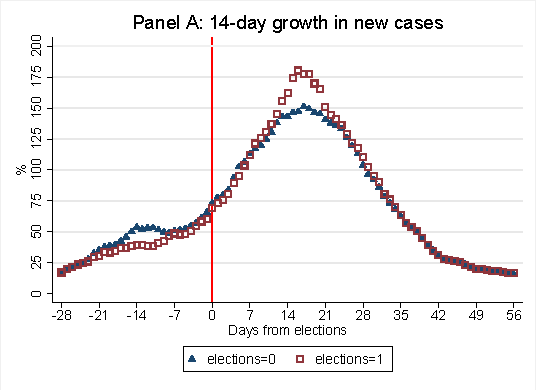
\includegraphics[scale=0.58]{binscatter_new_cases14.pdf} 
    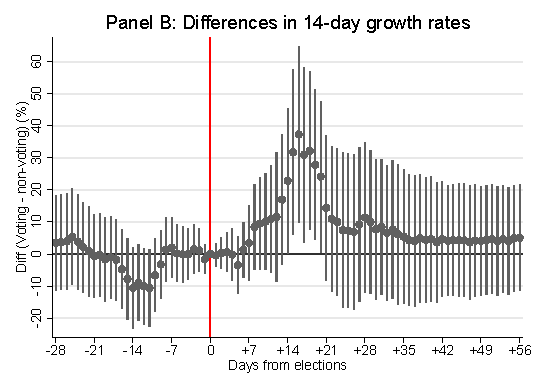
\includegraphics[scale=0.58]{Covid+_growth_rate14.pdf} 
	\caption{Volby a růst nových případů covid-19. (Panel A: Růst nových případů ve volebních a nevolebních obvodech. Panel B: Rozdíl růstu mezo volebními a nevolebními okrsky v procentech.)}
    \label{fig:Covid_growth14}
	\end{center}
\end{figure}

Tuto skutečnost potvrzuje i vývoj hospitalizací, jak je znázorňuje obrázek \ref{fig:hospit_growth}. Tato data ukazují, že rychlejší dynamika nových detekovaných případů ve volebních obvodech není nějakým umělým artefaktem, který by byl způsoben např. jinou strategií testování, ale že mu odpovídá i rychlejší růst hospitalizací. Obrázek  \ref{fig:hospit_growth} odpovídá předešlému obrázku pro nové případy, rozdílně zde uvádíme pouze 90\% intervaly spolehlivosti (výsledky hospitalizací jsou \uv{slabší} již z~povahy dat -- zatímco růst nových případů jsme schopni sledovat na úrovni všech 6259 obcí České republiky, v~případě hospitalizací máme pozorování řádově méně -- pouze na úrovni 206 obcí s~rozšířenou působností, na které je ČR rozdělena).

\begin{figure}[ht]    
    \centering
    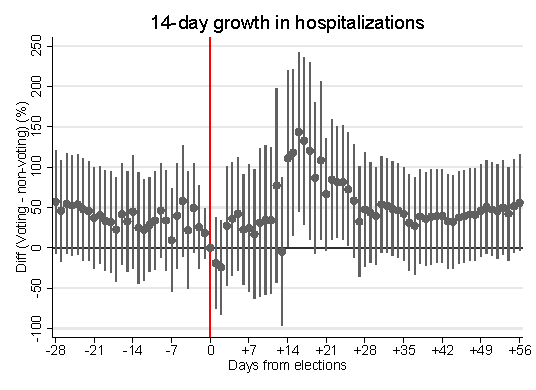
\includegraphics[scale=1]{Hospitalization_growth14.pdf}
    \caption{Volby a jejich vliv na růst hospitalizací. (Stejný princip jako Panel B na předešlém obrázku -- svislá osa představuje rozdíl mezi růstem hospitalizací ve volebních a nevolebních obvodech v procentech)}
     \label{fig:hospit_growth}
\end{figure}

\section*{Diskuse}
Vliv 2. kola senátních voleb na vývoj epidemie v~ČR byl dramatický. Je to výsledek do značné míry překvapivý, zejména pokud si uvědomíme, jak nízká je volební účast ve 2. kole senátních voleb v~porovnání s~účastí ve volbách do Poslanecké sněmovny Parlamentu ČR. Problémem ale není jen vliv voleb na vývoj epidemie, z~pohledu demokratické společnosti je stejně významný i opačný vliv, tedy vliv epidemie na volby. Je třeba si položit velice přirozenou otázku, a sice zda konání voleb v~průběhu epidemie nezmění jejich výsledek. Jelikož epidemie nezasahuje všechny věkové kohorty stejně, je třeba analyzovat růst nových případů separátně pro občany mladší a starší 65 let (občany podle tohoto měřítka rozdělují i veřejně přístupná data ÚZIS). Výsledek shrnuje obrázek  \ref{fig:heterogen_age}. Panel A~na tomto obrázku popisuje rozdíly čtrnáctidenního růstu epidemie mezi volebními a nevolebními obvody pro občany mladší 65 let, panel B pak stejné rozdíly pro občany starší 65 let. Mimo odhadnuté rozdíly pro jednotlivé dny ukazujeme i jejich 90\% intervaly spolehlivosti.

Vidíme, že signifikantní rozdíl mezi volebními a nevolebními obvody v~případě občanů starších 65 let vymizí. To je ovšem pouze částečně dobrá zpráva. Starší občané se sice úspěšně chrání tak, aby nebyli nakaženi v~průběhu volebního dne, nicméně cena, kterou za to všichni platíme z~pohledu reprezentativnosti demokratických voleb, je poměrně vysoká. 

Srovnáme-li krajské volby v~roce 2016 s~krajskými volbami 2020 (které proběhly společně s~1. kolem senátních voleb 2020, tedy také v~průběhu epidemie), vidíme velmi odlišnou účast voličů nad 65 let. Samozřejmě, z~principu tajných demokratických voleb nevíme přesně, kolik starších voličů se jednotlivých voleb zúčastnilo. Nicméně můžeme studovat závislost volební účasti v~jednotlivých volebních okrscích na podílu obyvatel starších 65 let. Skutečnost je taková, že v~krajských volbách v~roce 2016 každý 1 procentní bod podílu občanů starších 65 let zvyšoval volební účast o~0,511 procentního bodu (obecně se tedy občané nad 65 let účastnili v~krajských volbách velice nadprůměrně). Koeficient udávající vyšší volební účast v~okrscích s~vyšším počtem občanů nad 65 let klesl v~krajských volbách 2020 v~porovnání s~krajskými volbami 2016 na čtvrtinu a přestal být signifikantní.

Volby s~osobní účastí v~průběhu pandemie tak nejsou jen nebezpečné ve smyslu zrychlení dynamiky pandemie. Jejich problém spočívá i v~tom, že vzhledem k~různému nebezpečí nemoci covid-19 pro různé věkové skupiny nám volby v~průběhu pandemie nedávají skutečný obraz voličských preferencí tak, jak by byly zaznamenány v~dobách před epidemií. Hlas vyšších věkových skupin je proti předpandemické situaci slabší. V~tomto smyslu představuje pandemie další ohrožení demokracie. Tím totiž není jen přímé ohrožení životů jednotlivých občanů, ale i nepřímý vliv na zastoupení jejich hlasu v~demokratických volbách.

  
\begin{figure}[ht]
    \centering
    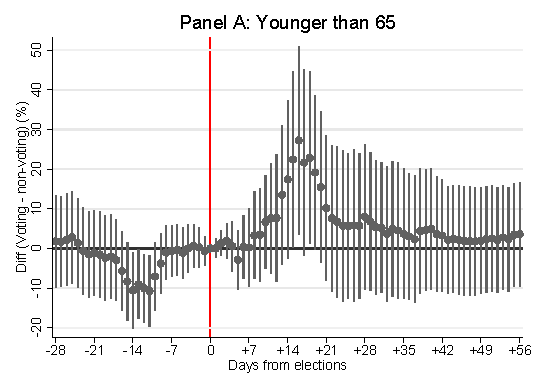
\includegraphics[scale=0.58]{Covid+_growth_rate14_less65.pdf} 
    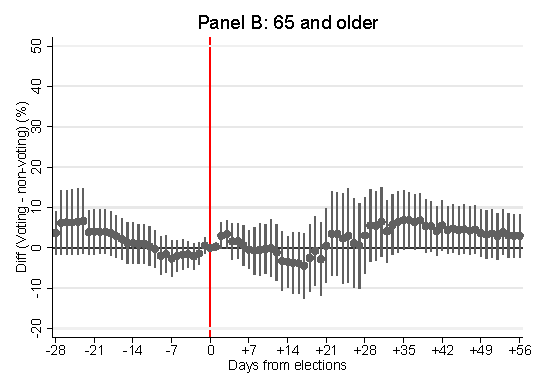
\includegraphics[scale=0.58]{Covid+_growth_rate14_older65.pdf} 
    \caption{Rozdíl růstu nových případů ve volebních a nevolebních obvodech rozdělen podle věku. Občané mladší 65 let vlevo, občané starší 65 let vpravo.}
 \label{fig:heterogen_age}
\end{figure}

\it
Původní verze článku byla publikována jako
Palguta J, Levínský R, Škoda S. Do elections accelerate the COVID-19 pandemic?: Evidence from a natural experiment [published online ahead of print, 2021 Sep 17]. J Popul Econ. 2021;1-44. doi:10.1007/s00148-021-00870-1
